Definitely need this chapter if you're using any data from any sources. 

\section{This is how you do sections}

\subsection{And this is a subsection}



\begin{wrapfigure}{R}{0.6\textwidth}
    \begin{center}
    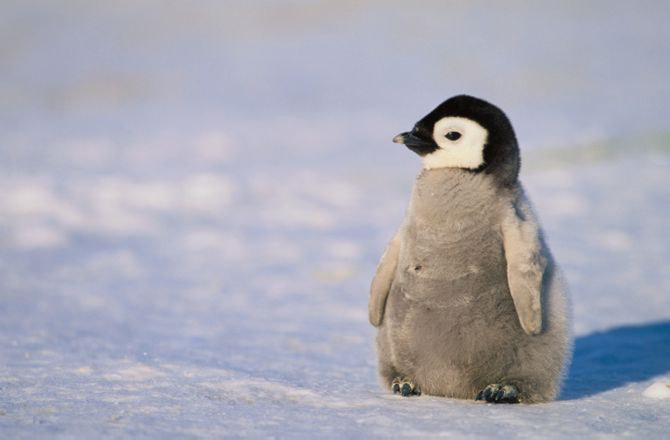
\includegraphics[width=\textwidth]{Chapters/Figures/FigureExample.jpeg}
    \caption{This is a figure caption. That is a penguin.}
    \end{center}
    \label{fig:penguin}
\end{wrapfigure}


Then you can refer to a figure in the text, like Figure \ref{fig:penguin}. 

\begin{table}[H]
    \centering
    \begin{tabular}{ccccccc}  
    \toprule
         Location & Track & Cycle & Seg & Laser&  Dates & Year\\ 
    \midrule
         Chukchi& 0381 & 14/15 & 05 & GT3L &    16 Jan/17 April& 2022 \\  
         Chukchi& 0373 & 14/15 & 03 & GT2L &  15 Jan/16 April& 2022 \\  
         Chukchi& 0373 & 14/15 & 03 & GT3L & 15 Jan/16 April& 2022 \\  
         Chukchi& 0815 & 14/15 & 03 & GT1L & 13 Feb/15 May& 2022 \\ 
         Chukchi& 0815 & 14/15 & 03 & GT2L & 13 Feb/15 May& 2022 \\  
         Beaufort& 0381 & 14/15 & 05 & GT1L & 16 Jan/17 April& 2022 \\ 
         Beaufort & 0320 & 14/15 & 05 & GT3L & 12 Jan/13 April & 2022 \\
    \bottomrule
    \end{tabular}
    \caption{This is what tables look like}
    \label{tab:icesattracks}
\end{table}
